% @Author: YangZhou
% @Date:   2017-06-20 20:27:38
% @Last Modified by:   YangZhou
% @Last Modified time: 2017-12-07 14:28:22

\documentclass[aps,prb,twocolumn,showpacs,amsmath,amssymb]{revtex4-1}

\preprint{APS/123-QED}

\usepackage{graphicx}% Include figure filesxx
\usepackage{bm}% bold math
\usepackage{dcolumn}% Align table columns on decimal point
\usepackage{bm}% bold math

\usepackage{multirow}
\usepackage{epsfig}
\usepackage{amssymb}

\newcommand{\angstrom}{\mbox{\normalfont\AA}}

\begin{document}

\title{Anisotropic in-plane thermal conductivity observed in multilayer silicene}
\author{Yang Zhou${}^{1,3}$}
\author{Zhi-Xin Guo${}^{2,1}$}
\email{zxguo08@hotmail.com}
\author{Shi-You Chen${}^{1}$}
\author{Hong-Jun Xiang${}^{1}$}
\author{Xin-Gao Gong${}^{1,3}$}
\email{xggong@fudan.edu.cn}
\affiliation{
  ${}^1$Key Laboratory for Computational Physical Science (Ministry of Education), State Key Laboratory of Surface Physics and Department of Physics, Fudan University, Shanghai 200433, China\\
  ${}^2$Department of Physics, Xiangtan University, Xiangtan 411105, China\\
  ${}^3$Collaborative Innovation Center of Advanced Microstructures, Nanjing 210093, Jiangsu, China
}
\begin{abstract}
  The silicon materials present complex surface reconstructions, which are usually neglected for the thermal conductivity investigations due to their small specific surface area. However, the reconstruction effect can be significant when the material thickness becomes ultra thin, i. e., multilayer silicene. Here we systematically study the thermal conductivity of multilayer silicene by means of Boltzmann Transportation Equation (BTE) method.  We find that the thermal conductivity of multilayer silicene present significant surface-structure dependence. The thermal conductivity of bilayer silicene varies from $3.31$ W/mK to $57.9$ W/mK depending on the specific surface structures. We also find that the surface reconstruction induces unusual large thermal conductivity anisotropy, which reaches 70\%  for the flour-layer  $2\times1$ silicene.  The anisotropy decreases with silicene thickness increasing, owing to the significant reduction of the thermal conductivity in the zigzag direction and its slight increment  in the armchair direction.
  Finally, we find that both the phonon-lifetime  anisotropy and the phonon-group-velocity  anisotropy contribute to the thermal conductivity anisotropy for the multilayer silicene.
  This work could be helpful in the field of heat management, thermoelectric applications involving silicene and other multilayer nanomaterials  with surface constructions in the future.

  \begin{description}
    \item[Keywords]
          Thermal conductivity, multilayer silicene, surface reconstruction, anisotropy
  \end{description}
\end{abstract}

\maketitle

\section{INTRODUCTION}

Many theoretical and experimental results have shown that quantum confinement and surface effects could reduce thermal conductivity remarkably while remain the electric conductivity remain at a relatively high level, which made them great potential in the applications of thermoelectrics. For example, the experiment of Boukai \emph{et al}.\cite{Boukai2008} shows that by varying the nanowire size and impurity doping levels, ZT values of approximately 100-fold improvement over bulk Si are achieved over a broad temperature range. Hochbaum \emph{et al}.\cite{Hochbaum2008} also proposed a way of increasing ZT by controling the roughness of silicene nanowires. At present, the thermal conductivity of the silicon nanostructures, i. e.,  silicene nanowires\cite{Hochbaum2008,Yang2010,Shi2009,Boukai2008} and monolayer silicene\cite{Pei2013,Ng2013,Xie2014,Zhang2014,Liu2014,Wang2015,Zhang2015a,Chen2016} had been well studied. However, the thermal conductivity of multilayer silicene is still mysterious.
The combined effects of quantum size and surface reconstruction in multilayer silicene is expected to induce exotic thermal transport properties different from both monolayer silicene and bulk Si,  which may make it suitable for the thermoelectric applications. Since the the thermal conductivity of monolayer silicene and  bulk Si have been well explored, investigation on multilayer silicene is also helpful for understanding the thermal conductivity  evolution from two dimensional (2D) to three dimensional (3D) systems.

The existing research on thermal conductivity of  2D materials  mainly focus on the ones with weak Van der Waals(vdW) interlayer interaction where there is no surface reconstruction, such as multilayer graphene\cite{Lindsay2011,Ni2012,Wang2011}, $MoS_2$\cite{Liu2015}, and black phosphorus\cite{Zhang2015,Peng2015,Jain2015}.  Whereas, the thermal conductivity of 2D materials with strong interlayer interactions have been barely explored.
The multilayer silicene which has been both theoretically predicted and experimentally synthesized can be an ideal material for such an investigation
\cite{Fu2014,Padova2016,Guo2015Structural}.
Previous studies  showed that the mutilayer silicene exhibit special surface reconstructions which induces the intriging electronic properties\cite{Fu2014,Guo2015Structural}. Naturally, one can expect that  the surface reconstruction is a significant factor for the thermal conductivity.
Especially, revealing the surface reconstruction effect on thermal conductivity anisotropy  in mutilayer silicene  promotes the applications of covalently bonded 2D materials in the thermoelectrics.

In this work, we systematically study the in-plane thermal conductivity of multilayer silicene with various thickness  (2-10 atomic layers) and surface reconstructions in use of  the BTE method.  We find that the thermal conductivity of multilayer silicene is significantly affected by the surface reconstructions, which can induce  either ultralow thermal conductivity value ($3.3$ W/mK) or unusual high thermal conductivity anisotropy (70\%).  This feature shows that the  multilayer silicene is an ideal candidate in the thermoelectrics.


\section{COMPUTATIONAL DETAILS}

The thermal conductivity of multilayer silicene structures are studied with the BTE method realized in ShengBTE\cite{Li2014}. In order to save the computing expense, the latest classical Mod potential\cite{Parks2007} based on the large scale parallel and efficient LAMMPS molecular dynamics software package is chosen\cite{Kumagai2007Development}. This potential is able to reconstruct the silicene material elastic constants, the melting point and phase transition. The Mod potential is constructed for different type of silicene structures by fitting its bond angle parameter to give correct melting point and elastic constants and is constructed referring the correction of the equilibrium bond length based on the experimental diamond structure and leads to smaller binding energy than that predicted by the first principle method.

The atomic models for multilayer silicene are shown in FIG.\ref{fig:structures}, which are adoped from recent work of Guo \emph{et al}\cite{Guo2015Structural}. For convenience, we define the names of these structures as "nlxs", where "n" is a pure number, representing the number of layers, "l" represents layer, "x" distinguishes different structures (concrete 1, 2, 3 etc. ) and "s" indicates the type along the length direction which is a (armchair) or z (zigzag). We show in TABLE.\ref{tab:table1} the structure names and  the minimum repeat cell periodicities of the multilayer silicene.

\begin{figure}[b]
  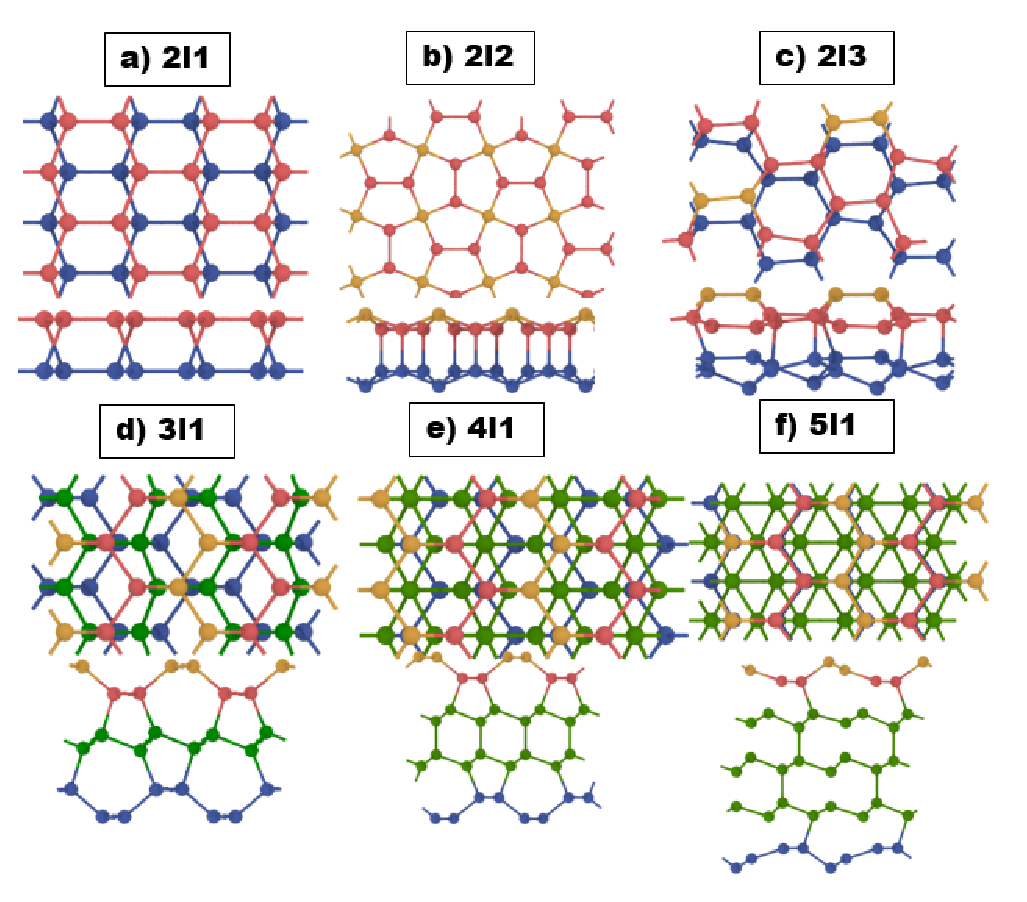
\includegraphics[angle= 0, width=0.95\linewidth]{structures.eps}
  \caption{\label{fig:structures}  (color online) Some typical structure of multilayer silicene. Within which  are top view and side view of the studied structures. The buckling atoms on the top surface are labeled as yellow while the red atoms represent the others on the top surface. All the atoms on the bottom surface are labeled as blue. The greens represent those that are inside the structure. The orientation of top view of the cells is labeled as arrows.}
\end{figure}

Before thermal conductivity calculation, the  structures are fully optimized using the conjugate gradient (CG) method to make them stable.  Then finite displacement method (FDM) realized in Phonopy\cite{Togo2008} and Thridorder respectively are applied to extract the second- and third-order force constants (FCs), in which hundreds of  slightly displaced supercells are generated. The obtained forces are calculated and used to calculate the FCs with numerical differential calculation. The chosen supercells are $3 \times 3 \times 1$ of premitive cells to make the in-plane dimension above 40 \angstrom, which ensures  the accuracy of calculated forces. Following to previous studies, we choose Si (111) layer spacing of $3.14 \angstrom$ as the interlayer thickness.

The thermal conductivity tensor can be calculated as

\begin{equation}
  \kappa^{\alpha\beta} = \sum_{k \sigma}{c_{k \sigma}v^{\alpha}_{k \sigma}v^{\beta}_{k \sigma}\tau_{k \sigma}} \label{eq:kappasum}
\end{equation}

where $c_{k \sigma}$ means the heat capacity of phonon mode,  $v_{k \sigma}^{\alpha}$ represents the mode group velocity, and $\tau_{k \sigma}$ is the phonon lifetime. The heat capacity is calculated with Eq.(\ref{eq:cv})

\begin{equation}
  c_{k \sigma}=\frac{\hbar \omega_{k \sigma} }{V} \frac{\partial f(\omega_{k \sigma},T)}{\partial T} \label{eq:cv}
\end{equation}

where $ f(\omega,T)=1/(exp(\frac{\hbar \omega}{k_b T})-1)$ is Bose-Einstein distribution function.

The calculations of $c_{k\sigma}$ , $v_{k \sigma}^{\alpha}$, and $\tau_{k\sigma}$ require the second- and third-order force constants (FCs) as inputs, where the detailed formulas are referred to the work of  Li \cite{Li2014}. To avoid underestimation of thermal conductivity, iteration method is used instead of relaxation time approximation (RTA). A $45\times 45 \times 1$ Monkhorst-Pack q-point mesh is used to obtain enough phonons for the convergence on the summation, as well as for their further statistical analytics.

\section{RESULTS AND DISCCUSION}

We first show that the surface reconstruction has substantial influence on thermal conductivity of the multilayer silicene.
FIG.\ref{fig:tc_length_sheng}(a) presents the length dependence of thermal conductivity of three bilayer silicene structures.
As one can see, thermal conductivity converges with cutoff phonon mean free path (MFP) very quickly in of 2l2  structure, while a little slower in the others. Moreover, the cutoff MFPs of 2l1 structure are very different in the armchair and zigzag directions. These features can be attributed to the different scattering intensity caused by the surface reconstructions.
It is known that the ballistic phonon transport is dominating  when a material length the is smaller than the MFP,  whereas the diffuse phonon transport is  dominating when a material length is larger than the MFP.
An empirical formula had been proposed by John A. Thomas\cite{Thomas2010}  to characterize the thermal conductivity of the phonon transport from ballistic to diffuse region, and accurately estimate thermal conductivity of the infinite long nanomaterials

\begin{equation}
  \kappa = \kappa_\infty (1-e^{-\frac{L}{L_c}}) \label{eq:eq_nemd}
\end{equation}

where $\kappa_\infty$ is the fitted full scattering thermal conductivity, $L_c$ is the transition length from the ballistic transportation to the diffuse transportation. Here we find that the length dependence of thermal conductivity of multilayer silicene can also be well described by this  formula.
The saturated thermal conductivity of 2l1 structure reaches up to 42.1 (57.9) W/mK in zigzag (armchair) direction, while it is  31.1 (31.1) W/mK  for 2l2 structure and  3.3 (5.6)  W/mK for 2l3 structure in zigzag (armchair) direction, confirming the significant influence of surface reconstruction on thermal conductivity.

The surface reconstruction also induces the thermal conductivity anisotropy, which can be estimated using
\begin{equation}
  \chi=\frac{|\kappa_{z,\infty}-\kappa_{a,\infty} |}{ max⁡(\kappa_{z,\infty}-\kappa_{a,\infty} ) } \times 100 \%  \label{eq:eq_chi}
\end{equation}
where $ \kappa_{z,\infty} (\kappa_{a,\infty})$ stands for the full scattering thermal conductivity (infinite thermal conductivity) in the zigzag (armchair) direction.
It is found that both 2l2 and 2l3 structures show large thermal conductivity anisotropy, i.e., 27\% and 41\%, respectively, while 2l2 structure does not exhibits the anisotropy owning to its rotational symmetry over $\pi/2$.  The ultra low and perticularly high anisotropy of thermal conductivity of bilayer silicene indicate its great potential applications in the thermoelectrics.


\begin{figure}[b]
  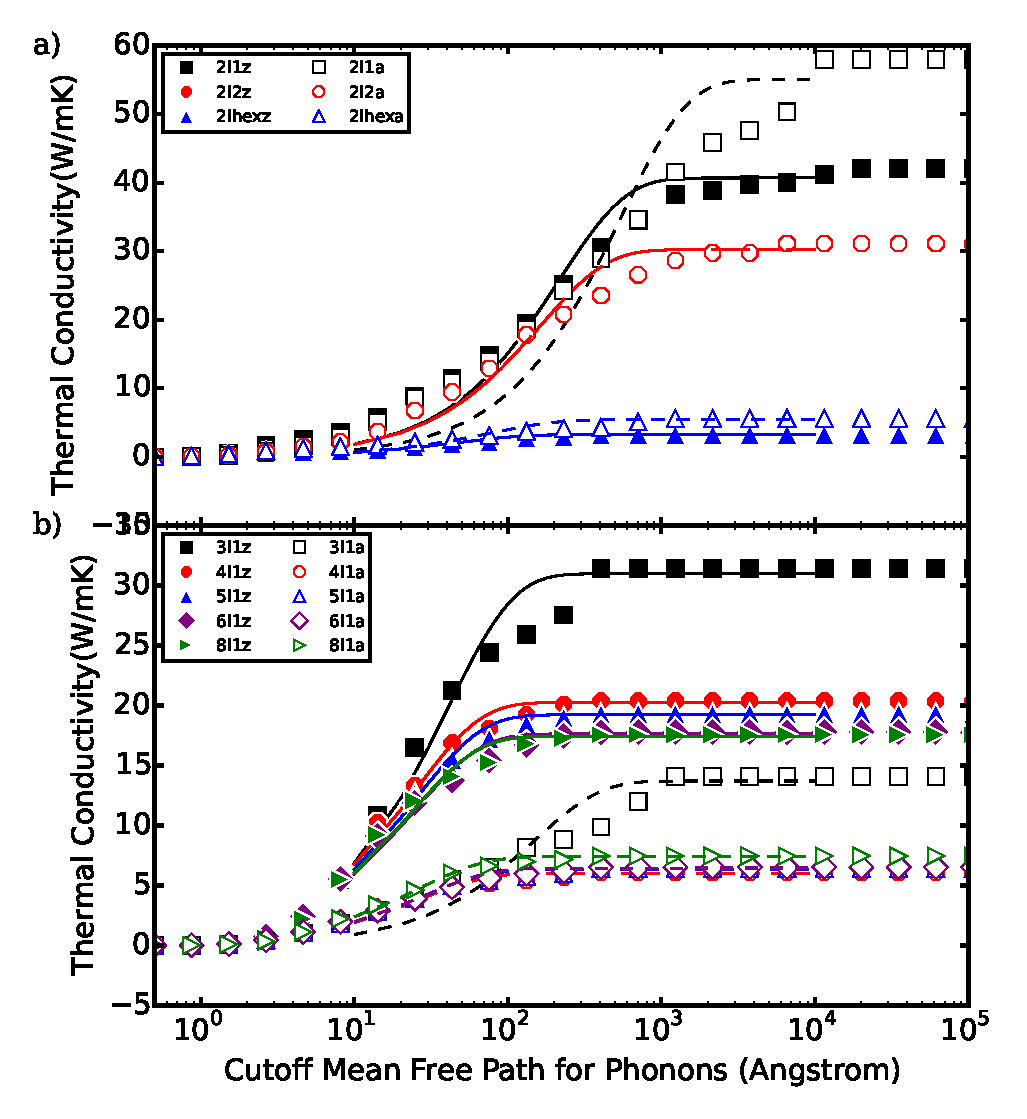
\includegraphics[angle= 0, width=0.9\linewidth]{tc_length_sheng.eps}
  \caption{\label{fig:tc_length_sheng} (color online) a) The thermal conductivity dependence on length for three types of bilayer silicene. b) The dependence on length of thermal conductivity for silicene with several layers.The scatters are the results of BTE calculations while the lines are fitted with Eq.(\ref{eq:eq_nemd}). The letter z/a in the legend mean the transport direction is zigzag/armchair. The dots of 2l2a and 2l2z are almost the same so red solid dots are covered. }
\end{figure}

\begin{figure}[b]
  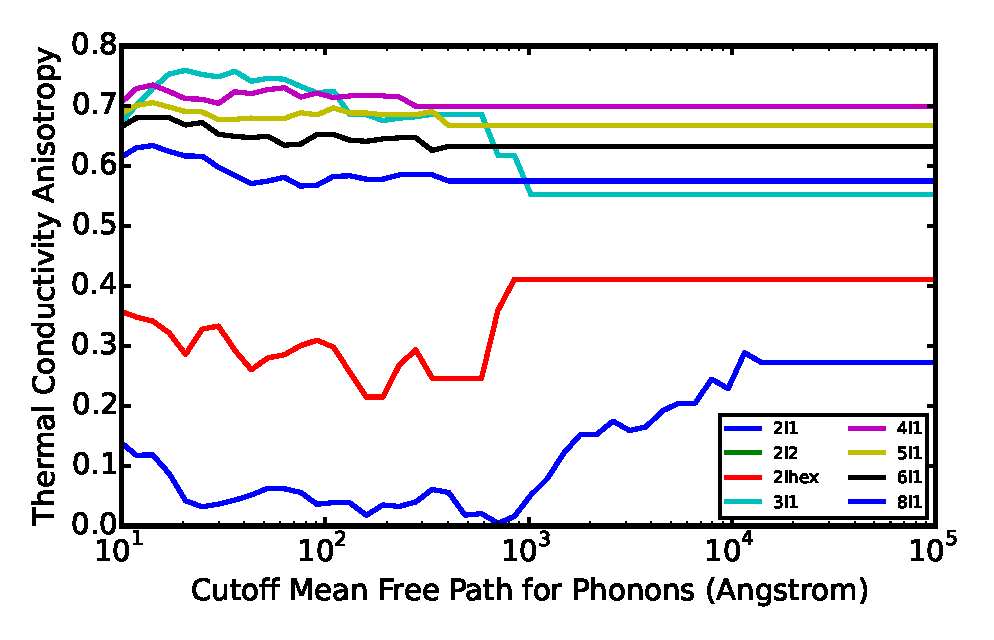
\includegraphics[angle= 0, width=0.9\linewidth]{chi.eps}{}
  \caption{\label{fig:chi} (color online) The anisotropy value dependence on length calculated with Eq.(\ref{eq:eq_chi})}
\end{figure}


We then discuss the thickness dependence of the thermal conductivity anisotropy. Here we mainly focus on the multilayer silicene with 3-8 atomic layers, whose surface presents the typical $2 \times 1$ Si(111) reconstruction.   A common feature is that the thermal conductivity in the zigzag direction ($\kappa_z$) is obviously  higher than that  in armchair ($\kappa_a$) direction, which induces anisotropy larger than 55\%.
The reason is that the zigzag direction of surface is composed of smooth zigzag atomic chains (as shown in FIG.\ref{fig:structures}), which are favorable for the heat transport. Whereas,  there are large geometry fluctuations in the armchair direction of the surface, which are unfavorable for the heat transport.
With the silicene thickness increasing from 4 to 8 atomic layers, the anisotropy monotonically decreases from 70\% to 58\%, showing the negative  effect of thickness on  thermal conductivity anisotropy. The negative  effect  is attributed to the decrease of $\kappa_z$ and increase of $\kappa_a$  with the  thickness increasing.
%This feature partially explains why the thermal conductivity  is almost isotropic in bulk Si, which usually has complex surface reconstructions. 
One exception is for the trilayer silicene, which has the largest thermal conductivity  but the smallest  anisotropy, compared to the thicker  $2\times1$ structures.  This could be understood by the direct interaction between the top and bottom layers, as well as the absence of ideal honeycomb ring under the surface layers, which is different from the thicker $2\times 1$ structures\cite{Guo2015Structural}.


We also investigated the size effect on the thermal conductivity anisotropy. As shown in FIG.\ref{fig:chi}, thermal conductivity of  2l1 bilayer silicene is almost isotropic  with length being 10-1000 \angstrom, and it becomes increasingly anisotropic with the length increasing  above 1000  \angstrom. This is essentially due to the difference of acoustic phonons in different directions,  which have large MFP.  As for the $2\times1$ structures with 3-8 Si layers in thickness, the high thermal conductivity anisotropy is obtained even when the length is as short as 10 \angstrom, implying that the anisotropy is  mainly attributed to the optical phonons. On the other hand, the thermal conductivity anisotropy of 2l3 silicene can be owning to both acoustic and  optical phonons in different directions.

\begin{table*}
  \caption{\label{tab:table1}
    The thermal conductivity and anisotropic ratio of different multi-layer silicene. Along with the average heat capacity ($kJ/m^3/K$) of zigzag direction and armchair direction. $Cv_z$ and $Cv_a$ correspond to the  heat capacity for thermal conductivity in  zigzag and armchair directions, respectively. }
  \begin{ruledtabular}
    \begin{tabular}{ccccccc}
          & Minimal period
          & $\kappa_{z,\infty}$
          & $\kappa_{a,\infty}$
          & $\chi$
          & $Cv_{z}$
          & $Cv_{a}$                                                           \\
      \hline
      2l1 & $1 \times 1$             & 42.10 & 57.92 & 27.31\% & 165.8 & 166.7 \\
      2l2 & $\sqrt{2}\times\sqrt{2}$ & 31.11 & 31.11 & 0    \% & 38.44 & 38.44 \\
      2l3 & $2 \times 2$             & 3.311 & 5.624 & 41.13\% & 22.42 & 22.42 \\
      3l1 & $2 \times 1$             & 31.44 & 14.05 & 55.29\% & 52.22 & 52.46 \\
      4l1 & $2 \times 1$             & 20.37 & 6.114 & 69.98\% & 37.71 & 37.89 \\
      5l1 & $2 \times 1$             & 19.33 & 6.419 & 66.78\% & 29.17 & 29.32 \\
      6l1 & $2 \times 1$             & 17.78 & 6.527 & 63.29\% & 23.73 & 23.86 \\
      8l1 & $2 \times 1$             & 17.56 & 7.461 & 57.51\% & 17.26 & 17.36 \\
    \end{tabular}
  \end{ruledtabular}
\end{table*}

To explore the origin of anisotropy, we have calculated the frequency distribution of thermal conductivity in armchair and zigzag directions  (Fig.\ref{fig:tc_freq}).
It is found that the  anisotropy is mainly attributed to the low-frequency (0-5 THz) phonons for the bilayer silicene, i. e., 2l1 and 2l3, where thermal conductivity in armchair direction is obviously larger than that of zigzag direction.
Whereas, for the $2\times1$ structures thicker than 3 Si layers, the thermal conductivity in armchair and zigzag directions is nearly the same in the low-frequency region, and the anisotropy is mainly  attributed to the high-frequency (5-20 THz) phonons.
In addition, the anisotropy of the 3l1 structure is resulted by the  phonons with frequency in range of 10-20 THz, below which the summation of contributions to thermal conductivity are nearly the same in armchair and zigzag directions.

To have a deep inside into the origin of anisotropy, it's helpful to investigate all the factors that contribute to thermal conductivity according to Eq.(\ref{eq:kappasum}).
We selected all the phonons along  $\Gamma\rightarrow X$ and $\Gamma \rightarrow Y$ directions in BZ, and calculated their heat capacity with Eq.(\ref{eq:cv}). The averaged heat capacity of silicene structures are shown in Table.\ref{tab:table1}, where $Cv_z$ and $Cv_a$ correspond to the  heat capacity for thermal conductivity in  zigzag and armchair directions, respectively.  As one can see, $Cv_z$ and $Cv_a$  strongly depend on the reconstruction-structure and thicknes of multilayer silicene, but their difference in the same structure is very small. This result shows that the thermal conductivity anisotropy is insensitive to the heat capacity.
%This is due to the insensitivity of heat capacity to frequency when the frequency is low and the value is ignorable when frequency is relatively high, which means when considering only acoustic phonons the heat capacity is close to constant.

\begin{figure}[b]
  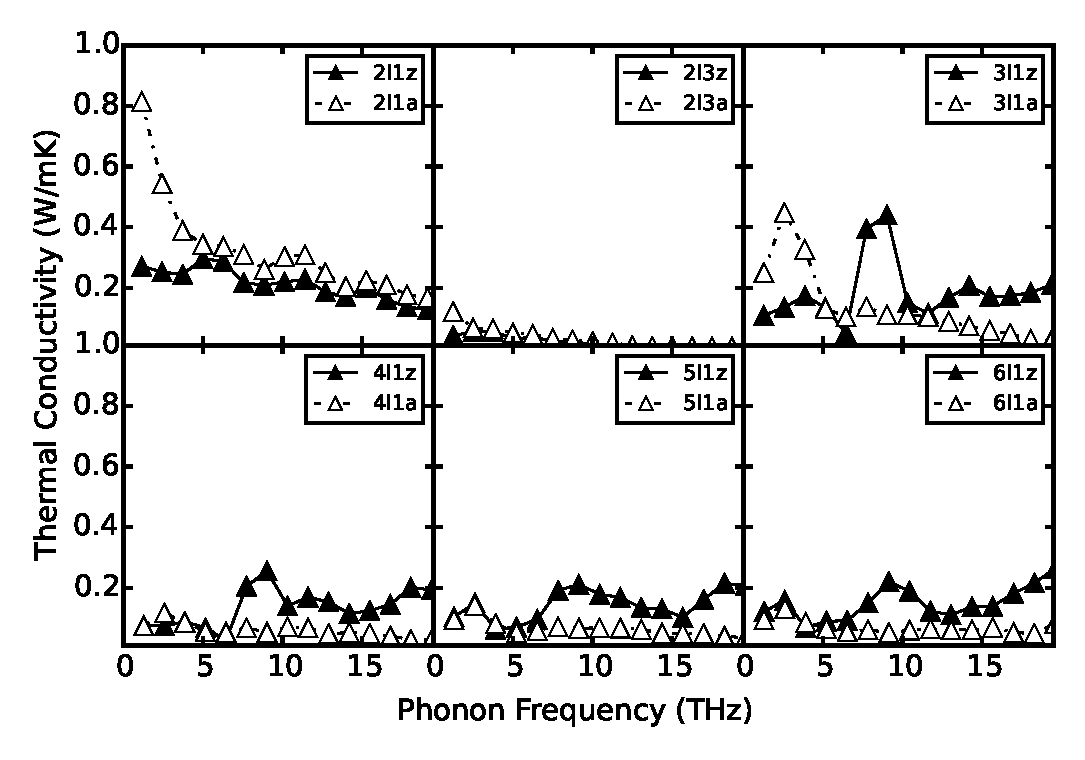
\includegraphics[width=0.9\linewidth]{tc_freq.eps}
  \caption{\label{fig:tc_freq} (color online)  The converged thermal conductivity versus phonon frequency of the structures. }
\end{figure}

\begin{figure}[b]
  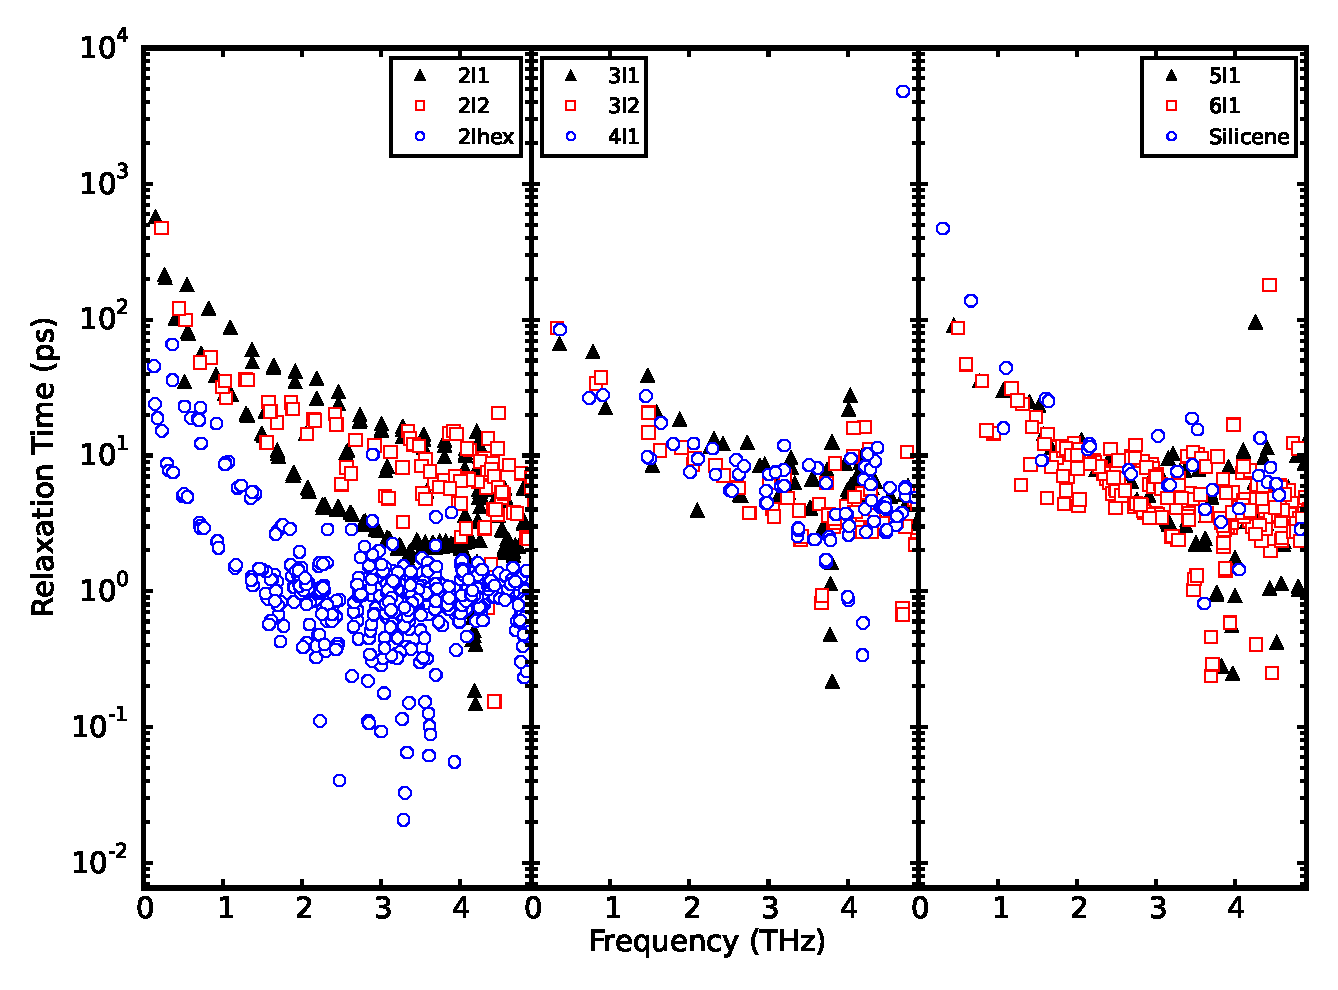
\includegraphics[width=0.9\linewidth]{tau.eps}
  \caption{\label{fig:tau} (color online) Lifetime of phonons considering three-phonon scattering for all the structures. }
\end{figure}

We then explore the contributions from the phonon lifetimes for the anisotropy.
We considered the three-phonon scattering process, where the phonon scattering rate could be obtained by the Fermi-golden rule\cite{Li2014} considering only the relaxation time approximation (RTA). The the iterative method was then used to include the cross influence of the phonon excitation, witch usually gives lager but more accurate lifetimes than the RTA. The frequency dependence of phonon lifetime calculated with ShengBTE\cite{Li2014} are shown in FIG.\ref{fig:tau}, where the values are averaged for frequency bins to reduce complexity.  It is shown that the lifetimes of larger than 1 ps for bilayer silicene structures (2l1, 2l3) distribute on the low-frequency region, indicating the dominating contributions of low-frequency phonons to the thermal conductivity. Moreover, the lifetime in armchair direction is obviously larger than that in zigzag direction in the low-frequency region. This feature inidcates that the anisotropy in bilayer silicene is attributed to the difference of phonon lifetimes in different directions.
On the other hand, the phonon lifetimes exhibit different frequency distributions in the thicker silicene, i. e.,  $2\times1$ structure with 3-6 Si layers, which cover both the low and high frequency regions with lifetimes  larger than 1 ps.  This is explains the high frequency phonons contribute significantly to the thermal conductivity in these structures (Fig. 4).  Except for the 4l1 structure, the lifetime distributions in zigzag and armchair directions are very similar for these  $2\times1$ structures, showing the tiny effect of phonon lifetimes on the anisotropy.


\begin{figure}[b]
  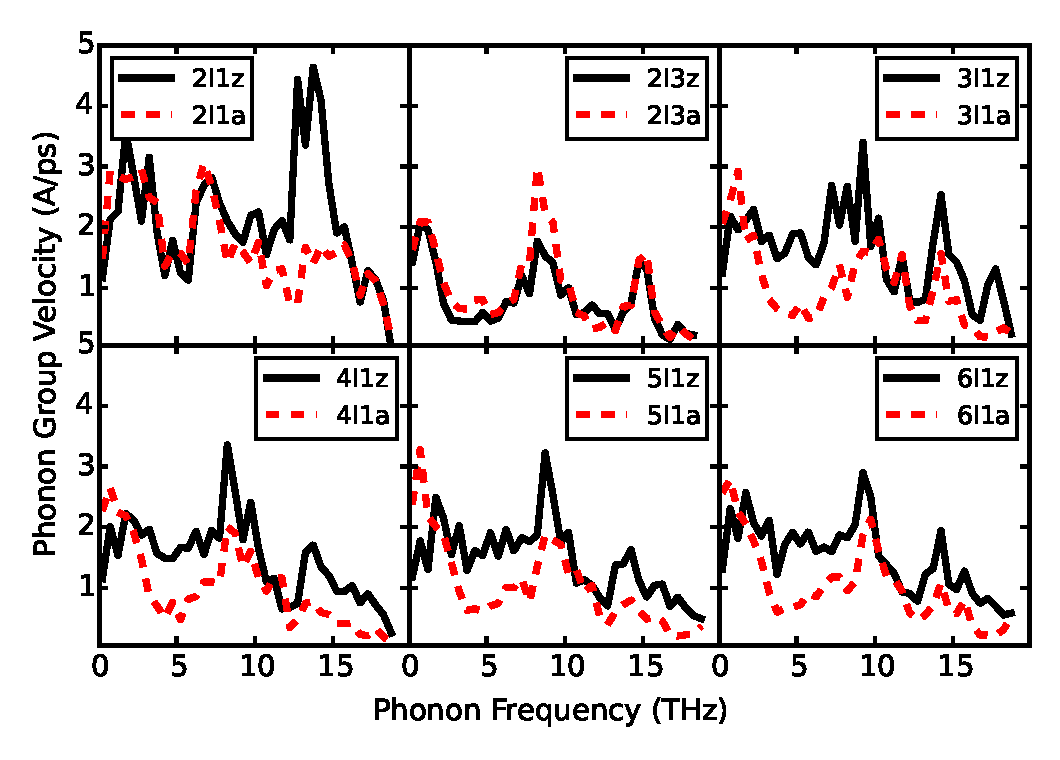
\includegraphics[width=0.9\linewidth]{gv.eps}{}
  \caption{\label{fig:gv} (color online)Group Velocity versus phonon frequencies for both zigzag direction and armchair direction of the structures.The histogram bin width is chosen as 1.5THz.}
\end{figure}

To further explore the origin of thermal conductivity anisotropy in multilayer  silicene, we have calculated the frequency dependence of phonon group velocities. As shown in Fig. 6,  the group velocity  difference is very small in the low-frequency region for the bilayer silicene, confirming that the anisotropy mainly comes from the different phonon scattering effect in armchair and zigzag directions,  which induce different phonon lifetimes.
As for the $2\times 1$ silicene with thickness more than layers,  the group velocity in zigzag direction is obviously larger than that in the armchair direction in most of the frequency region. Combined with the fact that the lifetime difference contributes little to the anisotropy for 3l1, 5l1, and 6l1 structures, one can conclude that the group velocity difference is the main reason for the anisotropy of $2\times 1$ silicene structures. It should be noted that the anisotropy of 4l1 structure is from contributions of both phonon lifetime and group velocity, which lead to its unusual large anisotropy up to 70\%.


\section{CONCLUSIONS}
By means of Boltzmann Transporation Equation methods, we have investigated thermal conductivity of multilayer silicene with various surface structures and thickness.
We found that the surface reconstruction has significant effect on thermal conductivity.  The smooth surface is favorable for heat conduction, while the rough surface greatly suppresses the heat conduction. Both ultra low (3.3 W/mK) and relatively high (57.9 W/mK) thermal conductivities have been obtained on bilayer silicene with different surface structures, which also induce large anisotropy of 41\% and 27\%, respectively. We also found that the $2 \times 1$  surface reconstruction induces the unusual large thermal conductivity anisotropy of 70\%  in the quadlayer silicene.  Moreover, we found that increasing silicene thickness, which has an effect of weakening the surface contribution to the thermal transport,  reduces the anisotropy. Finally, we clarify that the anisotropy of phonon lifetimes and phonon group velocities is the mainly contributes to   the thermal conductivity anisotropy for the bilayer and thicker $2\times 1$ silicene structures, respectively. Our results indicate that silicene structures with thickness of 2-4 layers present the most  exotic physical  properties, which may be a common feature for the 2D materials with strong interlayer interactions.
This work could be helpful in the field of heat management, thermoelectric applications involving silicene and other multilayer nanomaterials in the future.

\quad \\
\section{ACKNOWLEGEMENTS}
This paper was partially supported by the National Natural Science Foundation of China, the Special Funds for Major State Basic Research, the Foundation for the Author of National Excellent Doctoral Dissertation of China, the Program for Professor of Special Appointment at Shanghai Institutions of Higher Learning, and the Research Program of Shanghai Municipality and the Ministry of Education.


\bibliography{ref}
\end{document}
